\documentclass[12pt, a4paper]{report}

% --- Inclusion des configurations ---
% =====================================
% CONFIGURATION DES PACKAGES ET COULEURS
% =====================================

% --- Encodage et langue ---
\usepackage[utf8]{inputenc}
\usepackage[T1]{fontenc}
\usepackage[french]{babel}
% \renewcommand{\familydefault}{\sfdefault}  % Utilise Computer Modern Sans Serif (désactivé)
% \renewcommand{\sfdefault}{qag}  % Spécifie cmss comme police sans empattement (désactivé)

% --- Packages pour la mise en page et le contenu ---
\usepackage{graphicx}               % Pour inclure des images
\usepackage[a4paper, margin=2.5cm]{geometry} % Gestion des marges
\usepackage{amsmath, amssymb}       % Outils mathématiques avancés
\usepackage[
    hidelinks,
    pdftitle={TRENCHANT\_TROULLIER\_VIRQUIN\_GES7\_Projet},
    pdfauthor={TRENCHANT Evan, TROULLIER Laël, VIRQUIN Rudy},
    pdfsubject={Projet GE S7},
    pdfkeywords={génie électrique, projet S7, INSA Strasbourg, GES7},
    pdfcreator={LaTeX},
    pdfproducer={LaTeX}
]{hyperref}    % Pour les liens cliquables et métadonnées PDF
\usepackage{fancyhdr}               % Pour personnaliser les en-têtes et pieds de page
\usepackage{xcolor}                 % Pour utiliser des couleurs
\usepackage{tcolorbox}              % Pour créer des boîtes colorées
\usepackage{float}                  % Pour mieux placer les figures
\usepackage{caption}                % Pour personnaliser les légendes
\usepackage{subcaption}             % Pour des sous-figures
\usepackage{booktabs}               % Pour de jolis tableaux
\usepackage{titlesec}               % Pour personnaliser les titres de chapitres
\usepackage{lastpage}               % Pour obtenir le nombre total de pages
\usepackage{datetime}               % Pour le formatage des dates
\usepackage{pgfgantt}           % Diagrammes de Gantt
\usepackage{enumitem}               % Pour personnaliser les listes

% --- Configuration des listes ---
\setlist[itemize,1]{label=\textbullet}    % Premier niveau : bullet standard
\setlist[itemize,2]{label=\textendash}    % Deuxième niveau : tiret
\setlist[itemize,3]{label=$\ast$}         % Troisième niveau : astérisque
\setlist[itemize,4]{label=$\cdot$}        % Quatrième niveau : point centré

% Configuration de la table des matières (exclut les subsections)
\setcounter{tocdepth}{1}  % Seuls les chapitres et sections apparaissent dans la TOC

% Configuration des titres
\titleformat{\section}{\normalfont\large\bfseries}{\thesection}{1em}{}
\titleformat{\subsection}{\normalfont\normalsize\bfseries}{\thesubsection}{1em}{}

% --- Package CircuiTikz avec configuration spéciale ---
\usepackage{tikz}                   % TikZ doit être chargé avant circuitikz
\usepackage[siunitx]{circuitikz} % Configuration pour les diagrammes électriques
\usetikzlibrary{babel}

% --- Définition des couleurs personnalisées ---
\definecolor{INSAbleu}{RGB}{0, 70, 127}
\definecolor{boxgray}{gray}{0.95}
\definecolor{remindercolor}{RGB}{173, 216, 230}     % Bleu clair pour les rappels
\definecolor{conclusioncolor}{RGB}{220, 53, 69}     % Rouge pour les conclusions
\definecolor{conclusionbg}{RGB}{255, 240, 240}     % Fond rouge très clair
\definecolor{BLANC}{RGB}{255, 255, 255}            % Couleur blanche pour le pied de page

% --- Définition des modèles de boîtes colorées ---
\newtcolorbox{reminderbox}[1][Rappel]{
    colback=remindercolor!20,
    colframe=remindercolor!80,
    coltitle=white,
    colbacktitle=remindercolor!80,
    title=#1,
    fonttitle=\bfseries,
    rounded corners,
    boxrule=1pt,
    left=3mm,
    right=3mm,
    top=2mm,
    bottom=2mm
}

\newtcolorbox{conclusionbox}[1][Conclusion]{
    colback=conclusionbg,
    colframe=conclusioncolor,
    coltitle=white,
    colbacktitle=conclusioncolor,
    title=#1,
    fonttitle=\bfseries,
    rounded corners,
    boxrule=1pt,
    left=3mm,
    right=3mm,
    top=2mm,
    bottom=2mm
}

\newtcolorbox{infobox}[1][Information]{
    colback=INSAbleu!10,
    colframe=INSAbleu,
    coltitle=white,
    colbacktitle=INSAbleu,
    title=#1,
    fonttitle=\bfseries,
    rounded corners,
    boxrule=1pt,
    left=3mm,
    right=3mm,
    top=2mm,
    bottom=2mm
}

\newtcolorbox{classicbox}[1][Information]{
    colback=gray!10,
    colframe=gray!50,
    title=#1,
    fonttitle=\bfseries,
    rounded corners,
    boxrule=1pt,
    left=3mm,
    right=3mm,
    top=2mm,
    bottom=2mm
}
        % Packages et couleurs
% =====================================
% CONFIGURATION DE LA MISE EN PAGE
% =====================================

% --- Format de date DD/MM/YYYY ---
\newdateformat{ddmmyyyy}{\THEDAY/\THEMONTH/\THEYEAR}
\ddmmyyyy

% --- Personnalisation du format des chapitres ---
\titleformat{\chapter}
    {\normalfont\huge\bfseries}     % Format du titre
    {\thechapter~-~}                % Format du numéro (X - )
    {0pt}                           % Séparation entre numéro et titre
  {}                              % Code avant le titre
\titlespacing*{\chapter}{0pt}{-20pt}{20pt} % Ajustement des espaces : pas d'espace négatif avant le chapitre

% --- Configuration des en-têtes et pieds de page ---
\pagestyle{fancy}
\fancyhf{} % Nettoie les champs

% Configuration de l'en-tête
\fancyhead[L]{
\includegraphics[height=0.8cm]{images/logo_insa.jpg}}
\fancyhead[C]{\authorsInline}
\fancyhead[R]{\ddmmyyyy\today}

% Configuration du pied de page
\fancyfootoffset{0pt}
\fancyfoot[L,C]{}
\fancyfoot[R]{%
  \begin{picture}(0,0)
  % Réduction de l'image (scale passé de 1 à 0.8)
  \put(-13,-10){%
    
\includegraphics[scale=0.8]{images/foot-logo.png}% 
  }%
  % Ajout de \footnotesize pour réduire le texte
  \put(9.7,0){%
    \begin{minipage}{12mm}
      \centering
      \color{BLANC}{\footnotesize\thepage/\pageref*{LastPage}}% 
    \end{minipage}%
  }%
\end{picture}%
}

% Configuration des lignes de séparation
\renewcommand{\headrulewidth}{0.4pt}
\renewcommand{\footrulewidth}{0pt}

\addtolength{\topmargin}{-5pt}


% --- Configuration du style plain pour table des matières et chapitres ---
\fancypagestyle{plain}{%
  \fancyhf{} % Nettoie les champs
  % En-tête identique au style fancy
  \fancyhead[L]{
\includegraphics[height=0.8cm]{images/logo_insa.jpg}}
  \fancyhead[C]{\authorsInline}
  \fancyhead[R]{\ddmmyyyy\today}
  % Pied de page identique au style fancy
  \fancyfootoffset{0pt}
  \fancyfoot[L,C]{}
  \fancyfoot[R]{%
    \begin{picture}(0,0)
  % Réduction de l'image (scale passé de 1 à 0.8)
  \put(-13,-10){%
    
\includegraphics[scale=0.8]{images/foot-logo.png}% 
  }%
  % Ajout de \footnotesize pour réduire le texte
  \put(9.7,0){%
    \begin{minipage}{12mm}
      \centering
      \color{BLANC}{\footnotesize\thepage/\pageref*{LastPage}}% 
    \end{minipage}%
  }%
\end{picture}%
  }
  \renewcommand{\headrulewidth}{0.4pt}
  \renewcommand{\footrulewidth}{0pt}
}

% --- Paramètres généraux de mise en page ---
\setlength{\parindent}{0pt}  % Suppression de l'indentation automatique des paragraphes

% --- Configuration de la numérotation des pages ---
% Commande pour démarrer la numérotation à 2 (page de garde = page 1 non numérotée)
\newcommand{\startpagenumbering}{%
    \setcounter{page}{2}%
    \pagestyle{fancy}%
}

% --- Configuration des titres de sections et sous-sections ---
% Chapitres et sections sans numérotation
\newcommand{\chapternn}[1]{\chapter*{#1}\addcontentsline{toc}{chapter}{#1}}
\newcommand{\sectionnn}[1]{\section*{#1}\addcontentsline{toc}{section}{#1}}
\newcommand{\subsectionnn}[1]{\subsection*{#1}\addcontentsline{toc}{subsection}{#1}}
\newcommand{\subsubsectionnn}[1]{\subsubsection*{#1}\addcontentsline{toc}{subsubsection}{#1}}

\titleformat{\section}{\normalfont\large\bfseries}{\thesection}{1em}{}
\titleformat{\subsection}{\normalfont\normalsize\bfseries}{\thesubsection}{1em}{}

% Numérotation des sections
\renewcommand\thesection{\arabic{section}.}
\renewcommand\thesubsection{\thesection\arabic{subsection}.}          % Mise en page et styles
% =====================================
% VARIABLES SPÉCIFIQUES AU PROJET
% =====================================

% --- Commandes modulaires pour le rapport (À MODIFIER POUR CHAQUE PROJET) ---
\newcommand{\tpnumero}{}
\newcommand{\tptitre}{Étude d'une cellule de commutation}
\newcommand{\tpauteurs}{
    \begin{tabular}{c}
        Estéban DUBOIS \\
        Rudy VIRQUIN
    \end{tabular}
}
\newcommand{\tpgroupe}{GE4}
\newcommand{\tpprofesseur}{Caio Augusto Fonseca De Freitas}
\newcommand{\tpdate}{\today} % Ou une date fixe: {30/09/2025}

% --- Page de garde personnalisée ---
\newcommand{\maketitlepage}{
    \begin{titlepage}
        \centering
        
\includegraphics[width=0.5\textwidth]{images/logo_insa.jpg}\par\vspace{1cm}
        {\Huge\bfseries Projet ENPU 2\par}
        \vspace{1.5cm}
        {\huge\bfseries \tptitre\par}
        \vspace{2cm}
        {\Large\itshape \tpauteurs\par}
        {\Large\itshape Groupe 2 \tpgroupe\par}
        \vspace{2cm}
        {\begin{figure}[H]
    \centering
    \begin{tikzpicture}
	% Paths, nodes and wires:
	\node[nigfete] at (8.98, 7.27){};
	\draw (9.48, 6.5) to[empty diode, l_={$T$}] (9.48, 8.04);
	\draw (9.48, 8.04) -| (8.98, 8.04);
	\draw (9.48, 6.5) -- (8.98, 6.5);
	\node[ieeestd buffer port](N1) at (7.152, 7){} node[anchor=south] at ([yshift=0.05cm]N1.north){$Driver$};
	\draw (2, 10) to[american voltage source] (2, 6);
	\draw (4, 10) to[capacitor] (4, 8);
	\draw (6.275, 7) to[square voltage source] (4, 7);
	\draw (4, 8) -- (4, 7);
	\node[ground] at (4, 6){};
	\draw (4, 7) -| (4, 6) -| (8.98, 6.5);
	\draw (8, 8.667) to[empty diode] (8, 10);
	\draw (9, 8.667) to[cute inductor, mirror, l_={$RL$}] (9, 10);
	\draw (8.98, 8.04) -| (9, 8.667);
	\draw (8, 8.667) -- (9, 8.667);
	\draw (4, 6) -- (2, 6);
	\draw (2, 10) -- (8, 10);
	\draw (8, 10) -- (9, 10);
	\node[circ] at (4, 10){};
	\node[circ] at (4, 7){};
	\node[circ] at (4, 6){};
	\node[circ] at (9, 8.667){};
	\node[circ] at (8, 10){};
\end{tikzpicture}
\end{figure}}
        \vfill
        {\large Professeur : \tpprofesseur\par}
        \vspace{0.8cm}
        {\large \tpdate\par}
    \end{titlepage}
} % Variables du projet

% =====================================
% DOCUMENT PRINCIPAL
% =====================================

\begin{document}

% --- Page de garde ---
\maketitlepage

% --- Démarrage de la numérotation à 2 (page de garde = page 1) ---
\startpagenumbering

% --- Introduction et objectifs ---
\chapter*{Introduction}
\addcontentsline{toc}{chapter}{Introduction}

Dans le domaine de l'électronique de puissance et de l'automatique, la commande des machines électriques constitue un enjeu majeur pour de nombreuses applications industrielles. Parmi ces machines, la machine à courant continu (MCC) occupe une place particulière de par sa simplicité de commande et sa capacité à fournir des couples élevés à basse vitesse.

Ce projet, réalisé dans le cadre du semestre 7 de la formation en Génie Électrique à l'INSA Strasbourg, porte sur l'étude et la réalisation de l'asservissement d'une machine à courant continu avec charge. L'objectif principal est de développer un système de contrôle permettant d'asservir précisément la vitesse et le courant de la machine tout en respectant les contraintes de performance imposées.

\section*{Contexte et problématique}

L'asservissement des machines électriques nécessite une approche méthodique combinant la modélisation théorique, la simulation numérique et la validation expérimentale. Dans le cas particulier de la machine à courant continu, plusieurs défis doivent être relevés :

\begin{itemize}
    \item La modélisation précise du comportement dynamique de la machine et de sa charge
    \item La conception de correcteurs adaptés pour les boucles de courant et de vitesse
    \item La limitation des dépassements lors des régimes transitoires
    \item L'optimisation des performances en régime permanent et dynamique
\end{itemize}

\section*{Objectifs du projet}

Ce projet vise à concevoir et valider un système d'asservissement complet pour une machine à courant continu. Les objectifs spécifiques sont les suivants :

\begin{enumerate}
    \item \textbf{Modélisation et simulation} : Développer un modèle mathématique précis de la machine à courant continu et de sa charge, puis l'implémenter dans les environnements MATLAB/Simulink et PSIM
    
    \item \textbf{Asservissement en courant} : Concevoir et régler une boucle de régulation de courant permettant de contrôler précisément le couple de la machine
    
    \item \textbf{Asservissement en vitesse} : Implémenter une boucle de régulation de vitesse en cascade avec la boucle de courant, utilisant soit un capteur tachymétrique soit un codeur incrémental
    
    \item \textbf{Respect des spécifications} : Garantir que les dépassements en vitesse et en courant restent dans la plage de 10 à 20\% lors des transitoires
    
    \item \textbf{Validation comparative} : Comparer les résultats obtenus entre les simulations MATLAB/Simulink et PSIM pour valider la cohérence des modèles
\end{enumerate}

\section*{Approche méthodologique}

La démarche adoptée suit une approche progressive et structurée :

\begin{itemize}
    \item \textbf{Phase 1} : Étude et modélisation de la machine seule
    \item \textbf{Phase 2} : Intégration de la charge mécanique et validation du modèle complet
    \item \textbf{Phase 3} : Conception et réglage de la boucle de courant
    \item \textbf{Phase 4} : Conception et réglage de la boucle de vitesse
    \item \textbf{Phase 5} : Optimisation globale et validation finale du système d'asservissement
\end{itemize}

Chaque phase fait l'objet d'une validation croisée entre les outils MATLAB/Simulink et PSIM, permettant de garantir la fiabilité des résultats et d'identifier d'éventuelles divergences de modélisation.

\newpage

% --- Sommaires ---
\tableofcontents
\newpage

% --- Cahier des charges ---
\section{Cahier des charges}
Le cahier des charges du projet est défini comme suit :
\subsectionnn{Asservissement en courant}
\begin{itemize}
    \item Temps de réponse maximal de 10 fois la periode de la MLI soit 0,45 ms
    \item Depassement maximal de 20\%
\end{itemize}

\subsectionnn{Asservissement en vitesse}
\begin{itemize}
    \item Depassement maximal de 20\%
\end{itemize}


% --- Inclusion des chapitres/parties du rapport ---
\chapter*{Planification du projet}
\addcontentsline{toc}{chapter}{Planification du projet}

La réalisation de ce projet d'asservissement d'une machine à courant continu nécessite une planification rigoureuse pour garantir l'atteinte des objectifs dans les délais impartis. Cette section présente l'organisation temporelle du projet et le diagramme de Gantt détaillant les différentes phases de développement.

\section{Diagramme de Gantt}

Le diagramme de Gantt ci-dessous illustre la planification détaillée du projet sur 14 semaines, avec les dépendances entre les tâches et les jalons importants.

\begin{figure}[H]
    \centering
    \begin{ganttchart}[
        vgrid,
        hgrid,
        x unit=0.8cm,
        y unit chart=0.7cm,
        title height=1,
        title label font=\footnotesize,
        bar label font=\footnotesize,
        group label font=\footnotesize,
        milestone label font=\footnotesize,
        bar height=0.6,
        group height=0.6,
        milestone height=0.6,
        bar/.append style={fill=INSAbleu!70},
        group/.append style={fill=INSAbleu!50},
        milestone/.append style={fill=red!70, rounded corners=2pt},
        progress label text={},
        link/.style={->, thick}
    ]{1}{14}
        
        % En-tête du diagramme
        \gantttitle{Planning Projet GE S7 - Asservissement MCC}{14} \\
        \gantttitle{Semaine}{14} \\
        \gantttitlelist{1,...,14}{1} \\
        
        % Phase 1 : Modélisation de base
        \ganttgroup{Phase 1 : Modélisation de base}{1}{3} \\
        \ganttbar{Étude théorique MCC}{1}{2} \\
        \ganttbar{Modélisation MATLAB}{2}{3} \\
        \ganttbar{Modélisation PSIM}{2}{3} \\
        \ganttmilestone{Validation modèle moteur seul}{3} \\
        
        % Phase 2 : Modélisation complète  
        \ganttgroup{Phase 2 : Modélisation complète}{4}{6} \\
        \ganttbar{Intégration charge mécanique}{4}{5} \\
        \ganttbar{Validation croisée MATLAB/PSIM}{5}{6} \\
        \ganttbar{Tests de robustesse}{6}{6} \\
        \ganttmilestone{Modèle complet validé}{6} \\
        
        % Phase 3 : Boucle de courant
        \ganttgroup{Phase 3 : Boucle de courant}{7}{9} \\
        \ganttbar{Conception correcteur courant}{7}{8} \\
        \ganttbar{Réglage et optimisation}{8}{9} \\
        \ganttbar{Validation spécifications}{9}{9} \\
        \ganttmilestone{Asservissement courant opérationnel}{9} \\
        
        % Phase 4 : Boucle de vitesse
        \ganttgroup{Phase 4 : Boucle de vitesse}{10}{12} \\
        \ganttbar{Conception correcteur vitesse}{10}{11} \\
        \ganttbar{Intégration boucles imbriquées}{11}{12} \\
        \ganttbar{Tests capteurs (tachy/codeur)}{11}{12} \\
        \ganttbar{Validation performance globale}{12}{12} \\
        \ganttmilestone{Système d'asservissement complet}{12} \\
        
        % Phase 5 : Finalisation
        \ganttgroup{Phase 5 : Validation finale}{13}{14} \\
        \ganttbar{Optimisation finale}{13}{13} \\
        \ganttbar{Documentation et rapport}{13}{14} \\
        \ganttbar{Préparation soutenance}{14}{14} \\
        \ganttmilestone{Projet finalisé}{14} \\
        
        % Liens entre les tâches
        \ganttlink{elem3}{elem5}
        \ganttlink{elem7}{elem9}
        \ganttlink{elem11}{elem13}
        \ganttlink{elem16}{elem18}
    \end{ganttchart}
    \caption{Diagramme de Gantt du projet d'asservissement MCC}
    \label{fig:gantt_projet}
\end{figure}

% --- Modelisation et simulation du moteur et du hacheur ---
\section{Modélisation et simulation du moteur et du hacheur}

\subsection{Modélisation du moteur à courant continu à vide}

\subsection{Modélisation du moteur à courant continu avec charge}

\subsection{Modélisation du moteur avec charge et hacheur}

% --- Asservissement du moteur ---
\section{Asservissement du moteur}

\subsection{Asservissement en courant du moteur}

\subsubsection{Modélisation sur Matlab/Simulink}

% image de l'asservissement en courant Simulink
\begin{figure}[H]
    \centering
    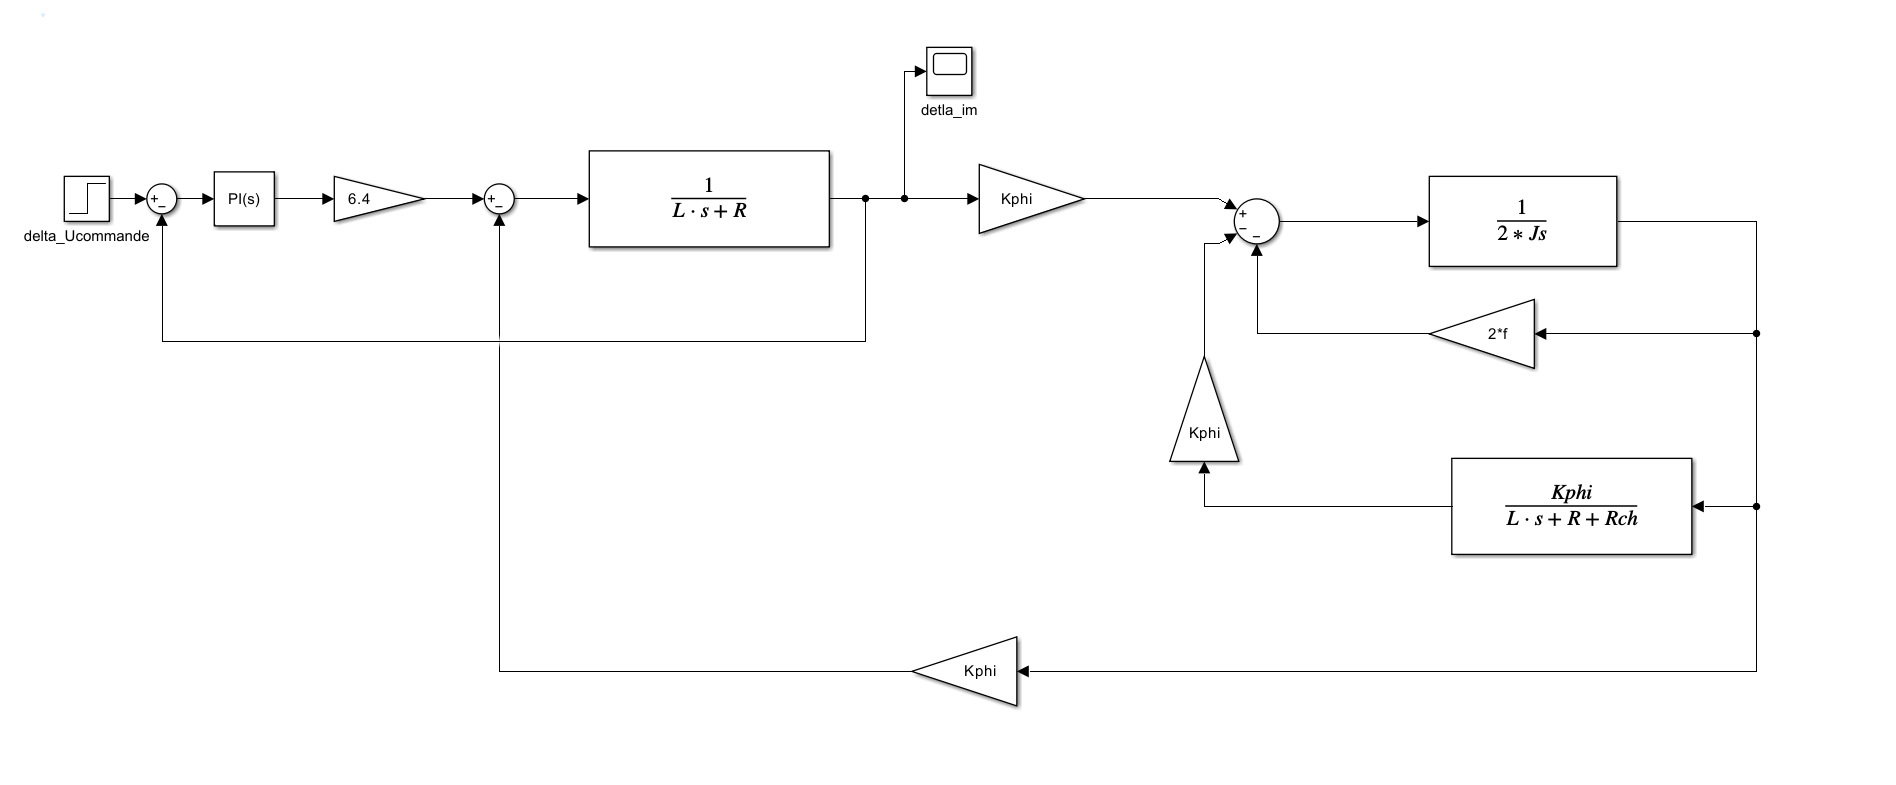
\includegraphics[width=1\textwidth]{images/boucle_de_courant/Simulink_boucle_de_courant.png}
    \caption{Schéma de l'asservissement en courant du moteur dans Simulink}
    \label{fig:asservissement_courant_simulink}
\end{figure}

% réponse indicielle de l'asservissement en courant Simulink
\begin{figure}[H]
    \centering
    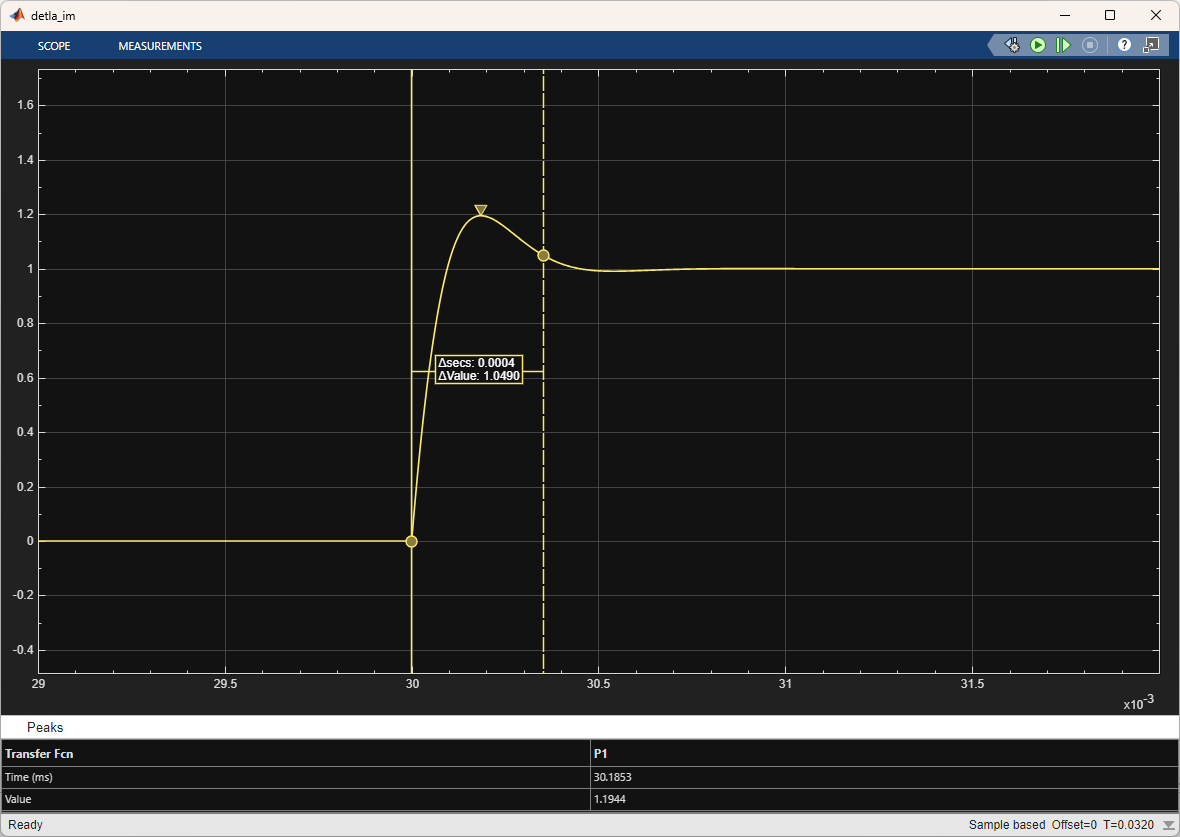
\includegraphics[width=1\textwidth]{images/boucle_de_courant/Simulink_reponse_indicielle_courant.png}
    \caption{Réponse indicielle de l'asservissement en courant du moteur dans Simulink}
    \label{fig:reponse_indicielle_courant_simulink}
\end{figure}

On constate que la réponse indicielle de l'asservissement en courant du moteur dans Simulink présente un dépassement d'environ 19\% et un temps de réponse de 0,35 ms. Ce qui respecte les spécifications du cahier des charges qui exige un dépassement maximal de 20\% et un temps de réponse maximal de 10 fois la prériode de la MLI soit 0,45 ms.

\subsubsection{Modélisation sur PSIM}

% image de l'asservissement en courant PSIM
\begin{figure}[H]
    \centering
    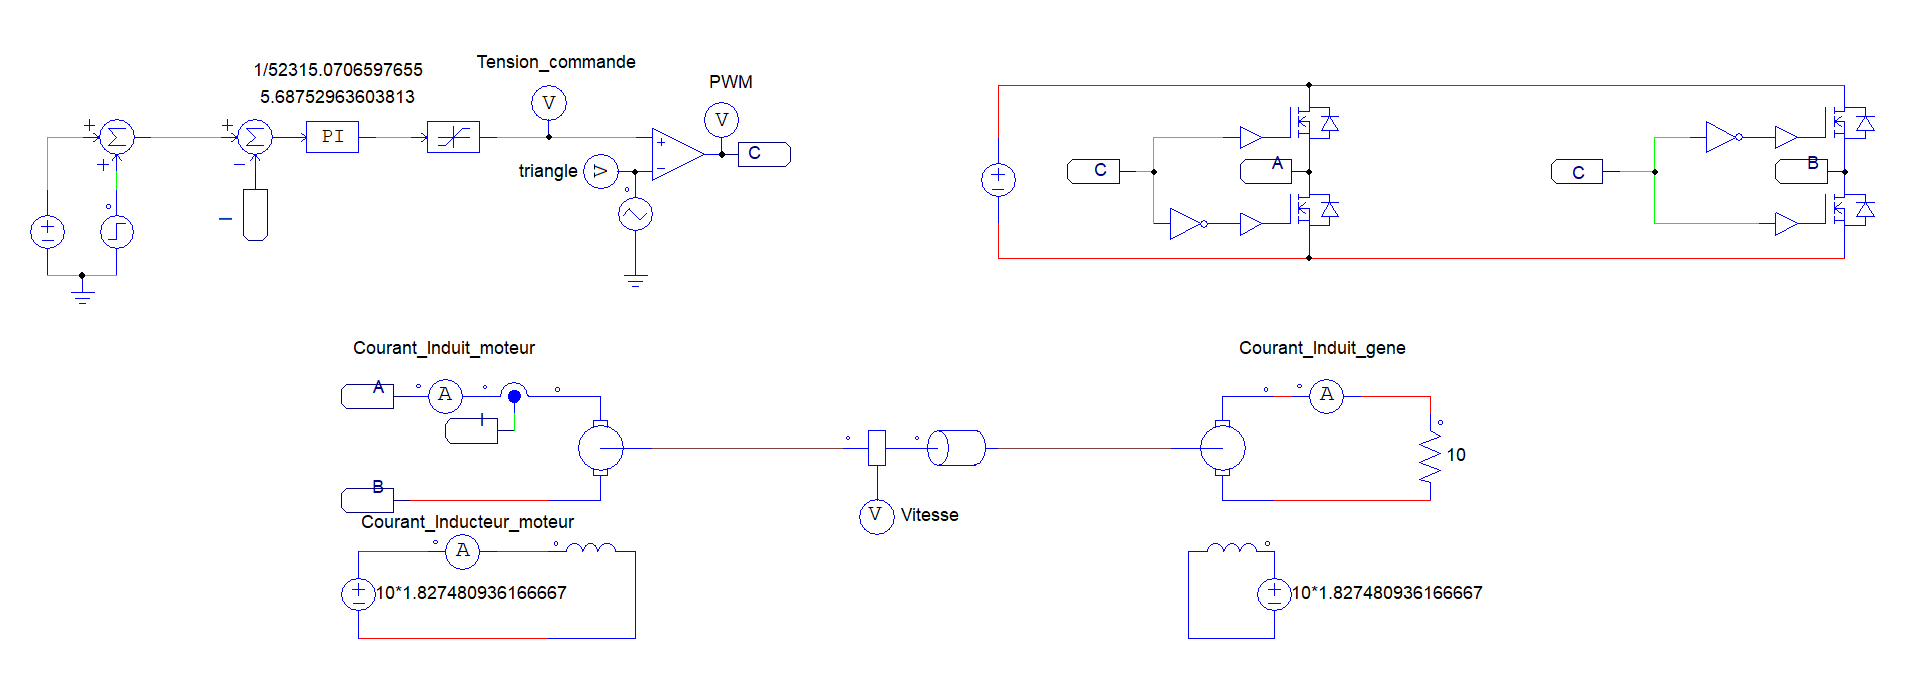
\includegraphics[width=1\textwidth]{images/boucle_de_courant/PSIM_boucle_de_courant.png}
    \caption{Schéma de l'asservissement en courant du moteur dans PSIM}
    \label{fig:asservissement_courant_psim}
\end{figure}
% réponse indicielle de l'asservissement en courant PSIM
\begin{figure}[H]
    \centering
    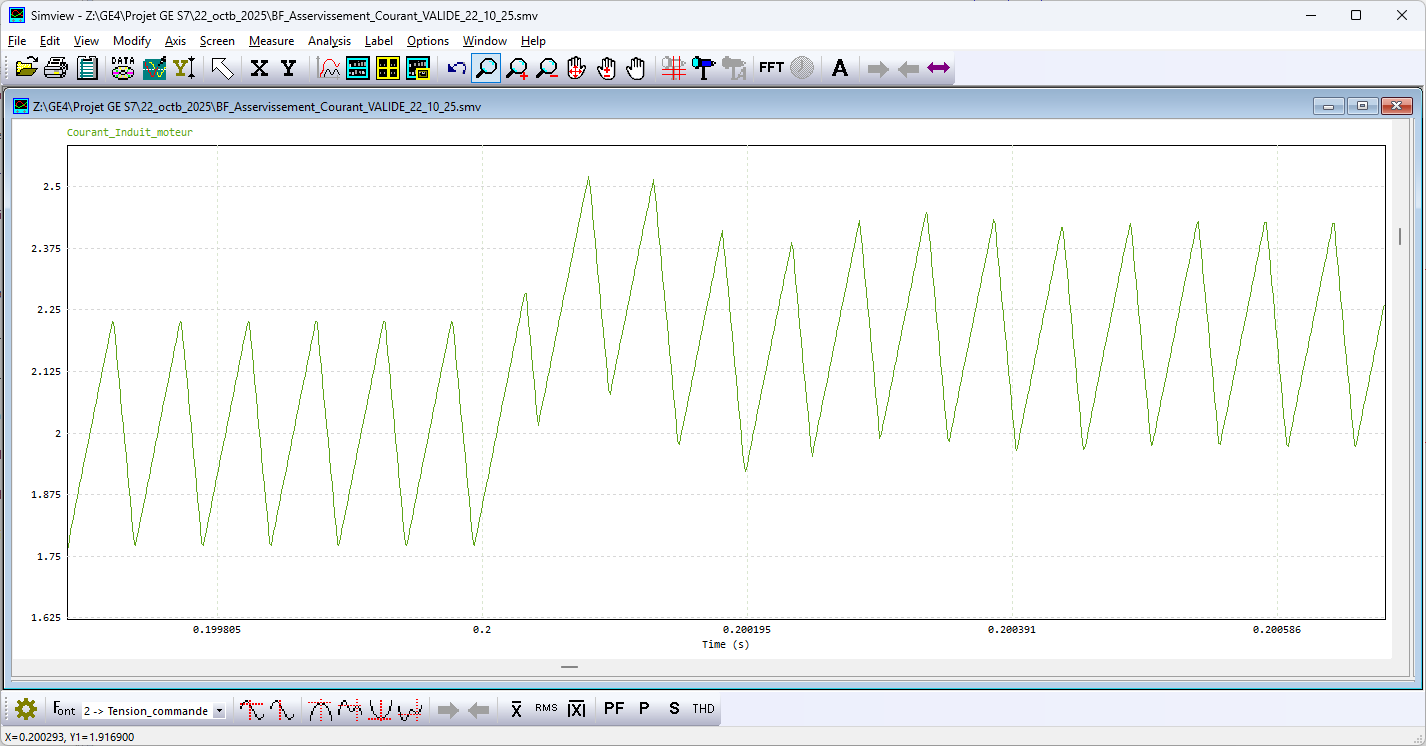
\includegraphics[width=1\textwidth]{images/boucle_de_courant/PSIM reponse indicielle courant BF.png}
    \caption{Réponse indicielle de l'asservissement en courant du moteur dans PSIM}
    \label{fig:reponse_indicielle_courant_psim}
\end{figure}

\subsubsection{Comparaison des résultats}

Dans cette section, nous allons comparer les résultats obtenus avec les deux outils de simulation, Simulink et PSIM.

% image de la comparaison des réponses
\begin{figure}[H]
    \centering
    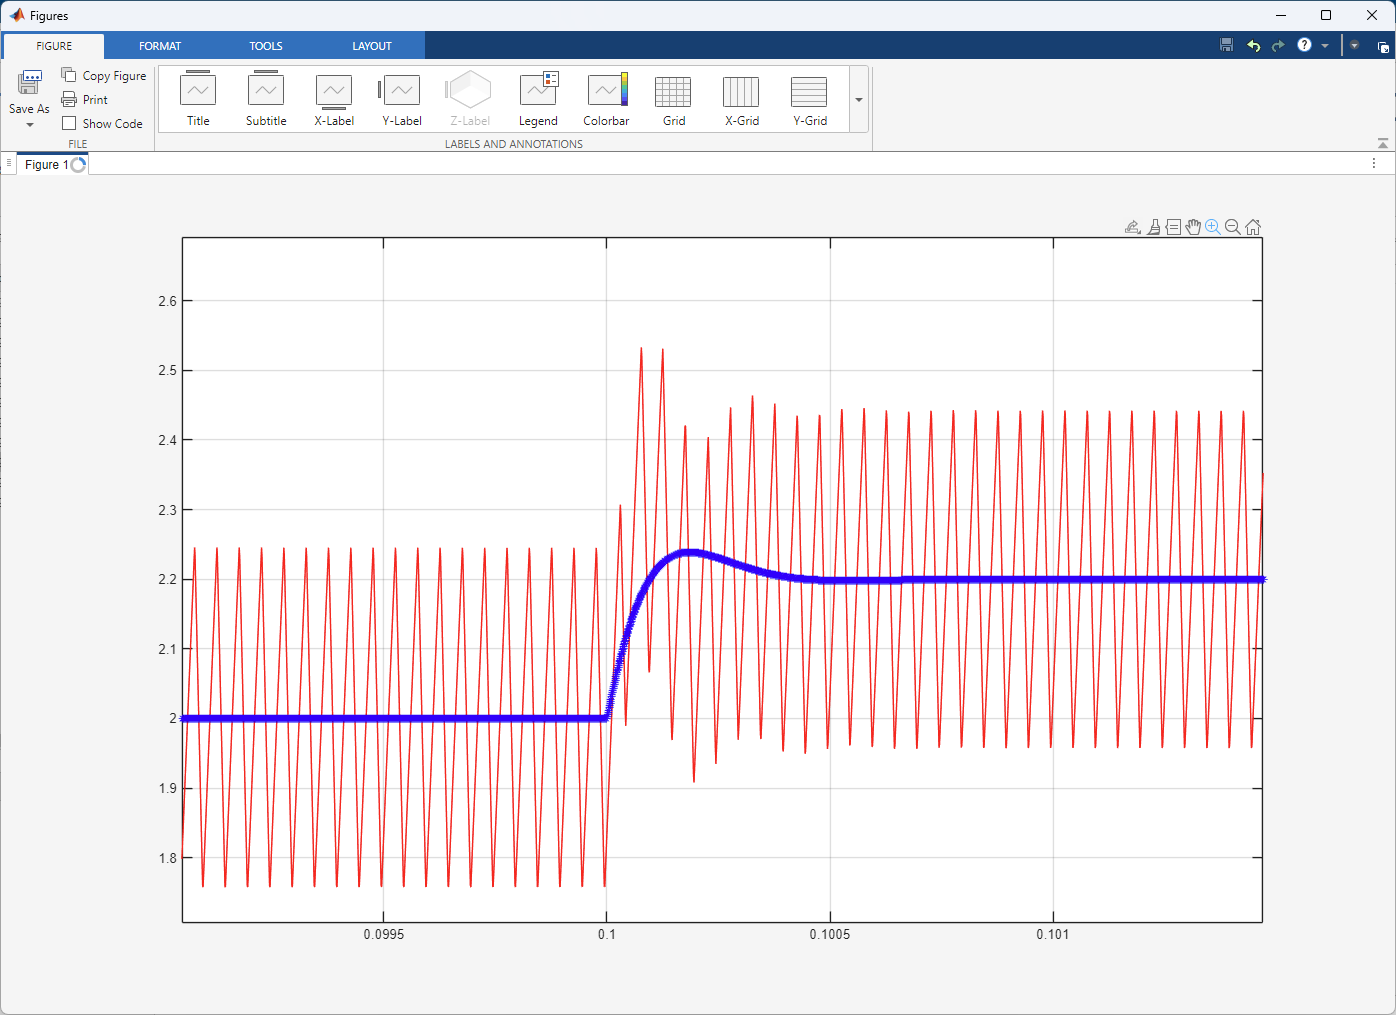
\includegraphics[width=1\textwidth]{images/boucle_de_courant/comparaison_reponse_indicielle_courant.png}
    \caption{Comparaison des réponses indicielle de l'asservissement en courant du moteur entre Simulink et PSIM}
    \label{fig:comparaison_reponse_indicielle_courant}
\end{figure}

\subsection{Asservissement en vitesse du moteur}

\subsubsection{Simulation sur Matlab/Simulink}
Nous commencons par la simulation de la vitesse du moteur en boucle ouverte sur Simulink. 

% réponse de l'asservissement en vitesse Simulink
\begin{figure}[H]
    \centering
    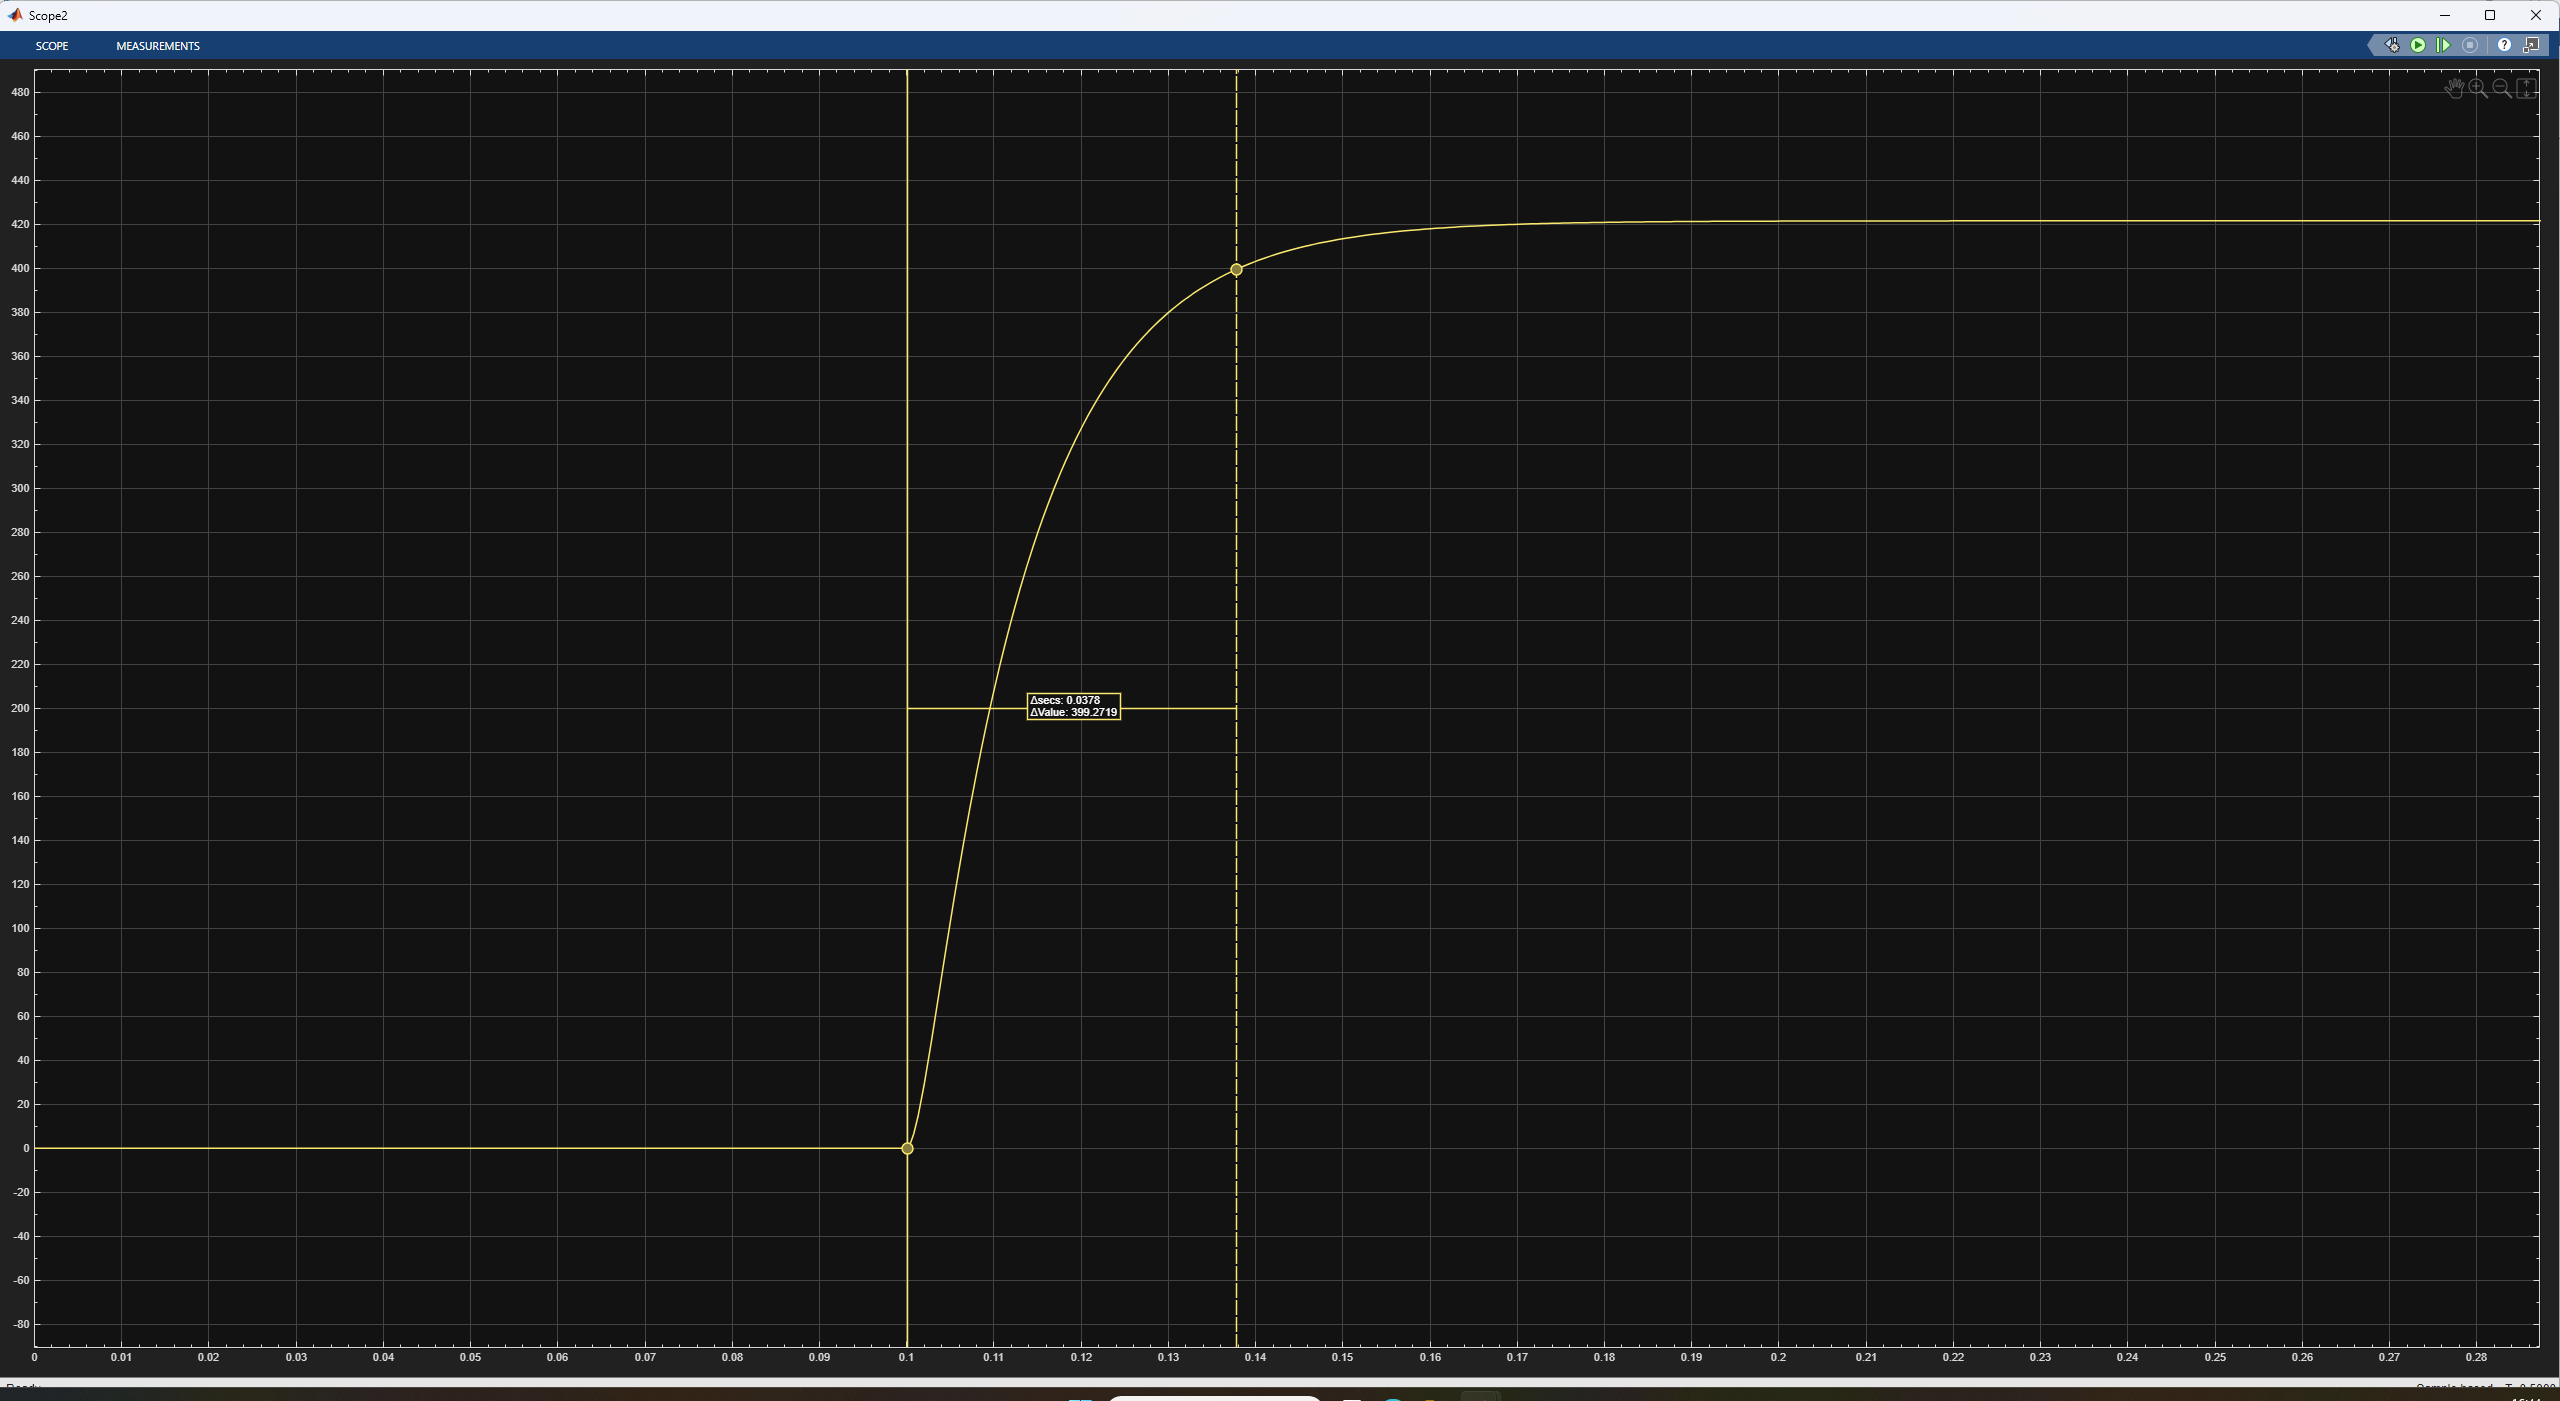
\includegraphics[width=1\textwidth]{images/asserv_de_vitesse_tachy/Vitesse_tr5_BO.png}
    \caption{Réponse de la vitesse du moteur en boucle ouverte dans Simulink}
    \label{fig:asservissement_vitesse_simulink}
\end{figure}
On releve un temps de réponse à 5\% en boucle ouverte pour la vitesse, sur Simulink : 37,8 ms

Nous cherchons ensuite à asservir la vitesse du moteur en boucle fermée avec un correcteur PI. Nous visons un temps de réponse à 5\% 3 fois plus rapide qu'en boucle ouverte soit 12,6 ms avec un dépassement maximal de 20\%.
\begin{figure}[H]
    \centering
    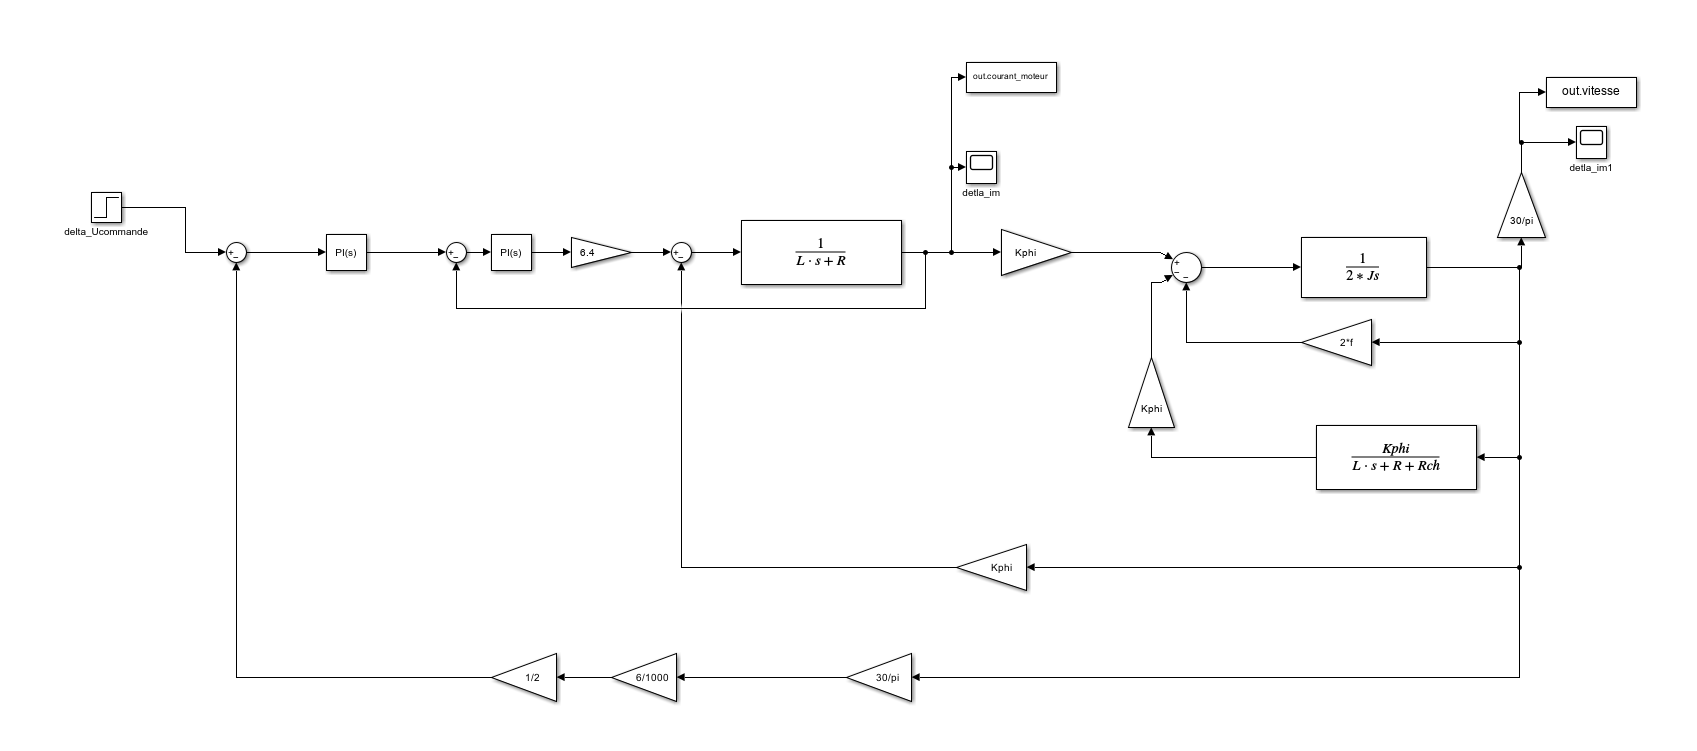
\includegraphics[width=1\textwidth]{images/asserv_de_vitesse_tachy/Simulink_boucle_de_courant_vitesse.png}
    \caption{Schéma de l'asservissement en vitesse du moteur dans Simulink}
    \label{fig:asservissement_vitesse_simulink_schema}
\end{figure}
A l'aide du PID Tuner de Simulink, nous obtenons les valeurs suivantes pour le correcteur PI :
\begin{itemize}
    \item Kp = 1,09577543479967
    \item Ki = 340,939693047362
\end{itemize}
% réponse de l'asservissement en vitesse Simulink
\begin{figure}[H]
    \centering
    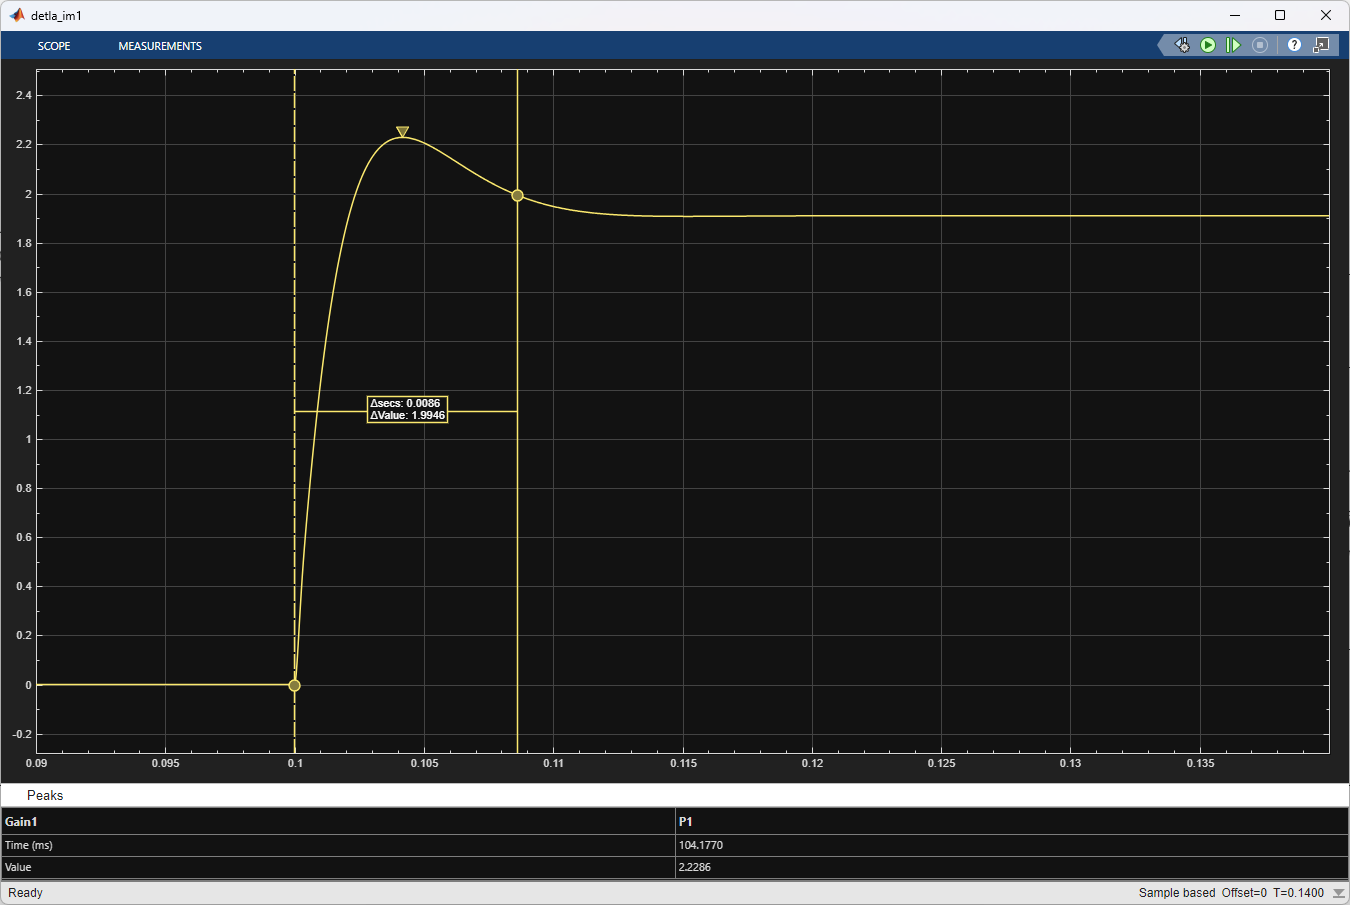
\includegraphics[width=1\textwidth]{images/asserv_de_vitesse_tachy/Vitesse_tr5_BF.png}
    \caption{Réponse de l'asservissement en vitesse du moteur dans Simulink}
    \label{fig:reponse_asservissement_vitesse_simulink}
\end{figure}
Nous relevons un temps de réponse à 5\% de 8,6 ms et un dépassement de 16,8\%, ce qui respecte les spécifications du cahier des charges.

\subsubsection{Simulation sur PSIM}

\subsubsection{Comparaison des résultats}

% Ajoutez ici vos autres chapitres avec \input{contenu/chapitre.tex}

\end{document}
